%%% mode: latex
%%% TeX-master: t
%%% End:

\chapter{基础理论与相关工作}
\label{cha:intro1}
%对比学习是自监督学习的重要途径,在计算机视觉、自然语言处理等诸多领域取得了瞩目的成就,推荐算法也根植于这一范式。正样本增强、负样本采样、损失函数设计,是对比学习的核心组件,也是提升推荐性能的关键途径。本章首先介绍对比学习的基本概念,并分析了推荐中的主流方法成对学习与对比学习的联系。然后介绍对比的研究现状,包括正样本的数据增强、负样本采样、网络架构设计以及损失函数设计。最后,介绍本文会使用到的一些重要的预备知识。

不完全标注的隐式反馈数据是制约推荐模型充分发挥潜力的瓶颈。自监督学习(SSL)\cite{Liu:2021:TKDE}作为一种学习范式,充分利用输入数据中的内在关系提取监督信号,可以减少对手动标签的依赖,广泛应用于推荐系统中最先进的推荐模型。本章首先从自监督学习的角度对推荐系统的现有工作进行梳理。其次对自监督推荐的主要途径--对比学习基础理论与相关工作进行介绍,并着重分析了成对损失BPR和对比损失InfoNCE之间的理论关联。最后,介绍本文会使用到的一些重要的预备知识。

\section{推荐算法相关工作}
近年来,借助深度神经网络模型的强大拟合能力和泛化性能,推荐系统取得了巨大的成功。然而,基于深度神经网络模型的推荐模型需要大量的训练数据。与可以通过众包完成的图像注释任务不同,推荐系统中的数据获取成本很高,因为个性化推荐依赖用户自身生成的数据,需要准确标注用户对海量物品的喜欢/不喜欢程度,才能使得推荐模型准确捕捉用户的偏好,从而产生准确的推荐。然而,大多数用户通常只与众多物品中的一小部分进行交互\cite{Steffen:2009:UAI,Zhang:2013:SIGIR}。因此,隐式反馈数据的稀疏性和标注不完全性问题成为制约深度推荐模型充分发挥潜力的瓶颈\cite{Zhang:2020:ACM}。

自监督学习(SSL)\cite{Liu:2021:TKDE}充分利用输入数据中的内在关系,通过对输入数据进行某种变换或处理提取监督信号,可以减少对手动标签的依赖,受到了相当大的关注。自监督学习的基本思想是通过精心设计的预训练任务(Pretext Task),例如对比语义相同的对象,从无标签数据中提取可迁移的知识。由于自监督学习有助于缓解服广泛存在的标签不足问题,已广泛应用于计算机视觉\cite{He:2020:CVPR,BYOL:2020:NIPS,Chen:2020:ICML},自然语言处理\cite{Devlin:2018:bert},音频表示学习\cite{Oord:2018:arxiv},图学习\cite{GCC:2020:KDD,velivckovic2018deep}等诸多领域。最新的基于自监督学习的方法甚至在许多计算机视觉(CV)和自然语言处理(NLP)任务中表现出与有监督模型相当的性能\cite{Robinson:2021:ICLR,Chuang:2020:NIPS,BYOL:2020:NIPS}。由于推荐系统的数据集标签不足,且受到自监督学习在其他领域取得的巨大成功的启发,目前已经有大量的研究探索将自监督学习应用于推荐领域。

自监督推荐(Self-Supervised  Recommendation,  SSR)模型为克服推荐系统中的数据稀疏问题提供了一种新的途径。本文综合文献\cite{Liu:2021:TKDE,SSR:2023:TKDE}的归纳,总结了自监督推荐(SSR)的三个关键特征如下:
\begin{enumerate}
\item \textbf{半自动地利用原始数据本身进行标注}。自监督推荐充分利用输入数据中的内在关系,通过对输入数据进行某种变换或处理来创建“伪标签”。例如BPR\cite{Steffen:2009:UAI}将交互的物品自动标记为正例,而未交互的物品标记为负例,就是执行自动化标注过程。需要注意的是,自动标注的标签是伪标签,不同于用户喜欢与否的真实偏好标签。

\item \textbf{通过提取自监督信号对推荐模型进行(预)训练的任务}。常见的自监督信号如“用户对正例的偏好强于负例”\cite{Steffen:2009:UAI},目的在于训练模型对正例的评分大于负例;另外一种常见的自监督信号是“用户物品二分图轻微扰动的语义不变性”\cite{lightgcl:2023:ICLR},目的在于训练推荐模型学习到用户物品二分图的结构信息。

\item \textbf{自监督任务旨在提升推荐性能,而非作为最终目标}。自监督任务引导的模型(预)训练阶段是为了编码用户物品的特征表示,与个性化推荐(下游任务)不一定一致。这一特征强调了推荐任务和自监督任务之间的主辅关系,学习良好的用户物品特征表示,是为了产生更准确的个性化推荐结果。例如,基于“用户对正例的偏好强于负例”的自监督信号设计的偏好对比任务,目标是激励推荐模型对正例评分大于负例评分,与推荐任务是一致的\cite{Steffen:2009:UAI,Jiancan:2022:arxiv}。而基于“用户物品二分图轻微扰动的语义不变性”这个自监督信号设计的图对比任务,目标是学习用户物品二分图的结构信息,与推荐任务不一致。因此图对比任务通常与偏好对比任务联合优化,并通过线性组合控制不同任务的主次\cite{10.1145/3543507.3583251,lightgcl:2023:ICLR}。
\end{enumerate}

推荐系统中涉及的自监督任务是多样的。根据自监督任务的性质,可以将现有的自监督推荐模型分为三种主要类型:对比型推荐算法、预测型推荐算法、生成型推荐算法。下文对这三种主要的自监督推荐算法进行介绍。
\vspace{-0.0011cm}
\subsection{对比型推荐算法}
\vspace{-0.0011cm}
典型的对比型推荐算法如图~\ref{2Fig:self1}所示,旨在通过拉近正样本对、推远负样本对,从而编码不同类别样本的差异特征。根据对比的目标不同,对比型推荐算法可以分为排序导向的偏好对比,和学习图结构信息导向的图对比。
%*******************************
\begin{figure*}[!]
	\centering
	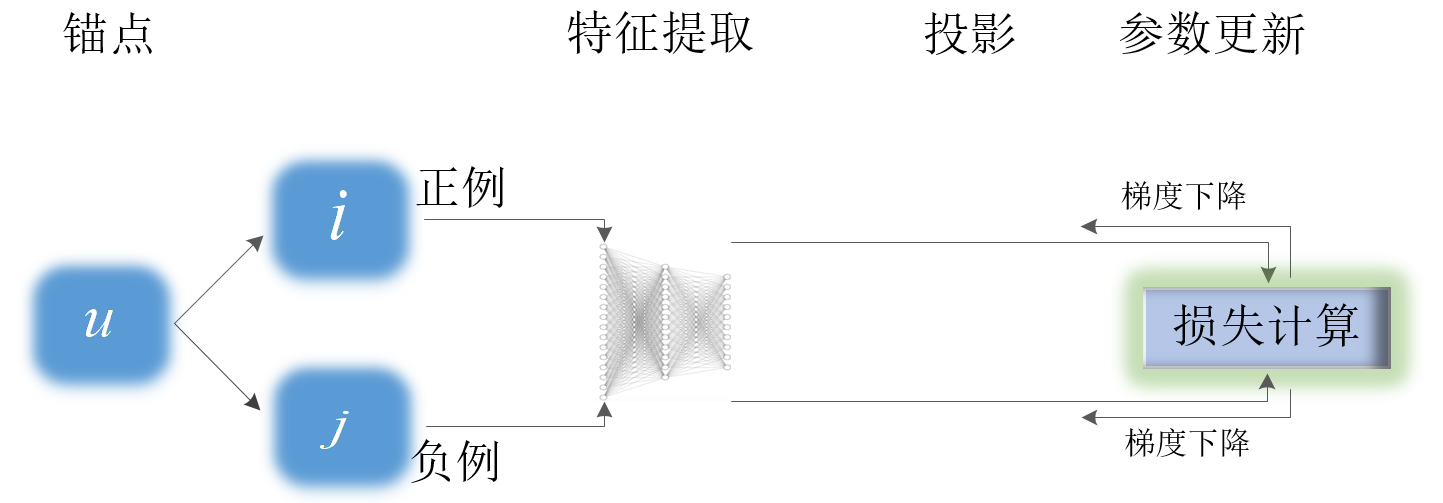
\includegraphics[width=0.8\textwidth]{self1.png}
	\caption{典型的对比型推荐算法示意图}
	\label{2Fig:self1}
\end{figure*}
%*******************************
\subsubsection{偏好对比}
偏好对比的自监督信号主要来自于用户对已交互物品的偏好大于未交互物品的偏好,开创性工作是成对学习BPR\cite{Steffen:2009:UAI},核心思想是通成拉近用户喜欢的正样本、推远用户不喜欢的负样本学习潜在的用户表示和物品表示。在偏好对比任务下,正样本的语义为用户喜欢的物品,负样本的语义为用户不喜欢的物品。这种基于偏好对比引导的模型(预)训练任务,激励推荐模型给正例评分大于负例,导致了排序列表的AUC指标的优化\cite{Steffen:2009:UAI}。随后InfoNCE损失\cite{Oord:2018:arxiv}也被广泛应用于偏好对比。文献\cite{Jiancan:2022:arxiv}揭示了在偏好对比任务下,优化InfoNCE损失有助于硬负例挖掘、缓解流行度偏差,并且优化排序列表的NDCG指标。由于BPR设计的偏好对比与下游排序预测任务具有一致性,逐渐主导了从隐式反馈数据中学习排序的任务\cite{Steffen:2014:WSDM,Xiangnan:2020:SIGIR,Wang:2019:SIGIR}。


偏好对比的后续的工作,主要是通过一些附属信息将正负样本对的概念进行拓展,构造了更具细粒度的偏好比较\cite{Weike:2013:IJCAI,Yu:2018:CIKM,Xiaoye:2011:MathProg,Xuejiao:2020:ASC,Qiu:2018:IS,Zhao:2019:FGCS}。例如,被购买的物品比只被浏览的物品更受用户喜欢\cite{Qiu:2018:IS};多次交互的物品比只有一次交互的物品更受用户喜欢\cite{Lerche:2014:RS};用户未看到过的物品应该比曝光给用户但没有交互的物品更受喜欢\cite{Wenhui:2019:WWW,Yu:2018:CIKM,Bin:2020:IS}。这些拓展的偏好比较实际上是通过附属信息提取了更密集和更可靠的自监督信号,有助于学习用户更具细粒度的偏好特征。


\subsubsection{图对比}
图(Graph)对比的自监督信号主要来自于用户物品二分图轻微扰动的语义不变性。在图对比任务下,正样本的语义为原图和增强图中的相同节点,负样本的语义为原图和增强图中的不同节点,目标是学习体现图结构信息的表示,与推荐任务不一致。根据对比的对象,遵循文献\cite{wu:2023:TKDE,gsl:2023:TKDE}提出的分类,图对比任务可以分为三种类型:结构级对比、特征级对比和模型级对比。
%尽管图对比在近年来研究较多,但由于图对比任务与推荐任务不一致,需要以偏好对比任务为主进行联合优化\cite{10.1145/3404835.3462862}。


%结构级对比的自监督信号主要来自于图结构扰动后的语义不变性,核心思想是:对图数据(Graph)进行轻微扰动,可能会导致类似的语义。通过对比不同的图数据,可以获得对结构扰动的共享不变性作为自监督信号。遵循文献\cite{wu:2023:TKDE,gsl:2023:TKDE}提出的分类法,将结构层对比分为两类:同尺度对比和跨尺度对比。同尺度对比涉及同一尺度上两个对象的视图,并进一步分为两个级别:局部-局部对比(Local-Local Contrast),全局-全局对比(Global-Global Contrast)。跨尺度对比涉及来自不同尺度上两个对象的视图,并进一步分为局部-全局对比(Local-Global Contrast)和局部-上下文对比(Local-Context Contrast)。

\textbf{结构级对比}的核心思想是:对图数据进行轻微扰动,可能会导致类似的语义\cite{10.1145/3459637.3482426,10.1145/3477495.3532009,liu2021contrastive,wang2023sequential,xia2021self,xie2022contrastive,liu2021contrastive,10.1145/3404835.3462862}。例如,SGL\cite{10.1145/3404835.3462862}将随机丢点/边和随机游走增强应对用户物品二分图进行增强,并使用共享的图LightGCN\cite{Xiangnan:2020:SIGIR}编码节点嵌入。例如,DCL\cite{liu2021contrastive}使用随机丢边来扰动节点的L跳领域,生成两个增强的邻域子图。然后最大化在这两个子图上学习到的节点表示之间的一致性,属于同尺度对比;例如,NCL\cite{lin2022improving}设计了一种原型对比目标,以捕捉节点与其原型之间的相关性。原型是通过使用K-means算法对所有用户或物品嵌入进行聚类获得的,并使用EM算法递归调整原型,属于跨尺度对比。


\textbf{特征级对比}的核心思想是:对特征或属性信息进行轻微扰动,可能会导致类似的语义。例如,SimGCL\cite{yu2022graph}和 XSimGCL\cite{yu2023xsimgcl}认为图数据增强对于推荐性能并不是必要的。图对比任务只是通过平滑学到的用户物品表示,缓解了流行度偏差,导致推荐模型泛化能力提升。基于这个发现,SimGCL添加随机噪声进行增强,从而得到更均匀的节点表示,提升推荐性能的同时缓解了流行度偏差问题。例如,MISS\cite{guo2022miss}认为直接扰动用户行为序列的数据增强方法,可能会改变数据的语义。基于此,该方法使用基于卷积神经网络的多兴趣提取器将包含行为数据和类别特征的数据转换为一组隐式兴趣表示,然后在特征级别上进行增强。

\textbf{模型级对比}的核心思想是:不同的模型架构,提取相同的数据输入得到的特征,可能会有类似的语义。这不同于前两个提取自监督信号的方式,结构级对比和特征级对比是从数据角度提取自监督信号,而模型级对比是动态修改模型架构以获取即时的增强视图。神经元屏蔽是一种常用的用于扰动模型的技术。典型的方法如DuoRec\cite{qiu2022contrastive},对基于Transformer的骨干网络应用不同的神经元屏蔽,进而获得两个模型级表示增强,通过模型级对比最大化两个表示之间的一致性。

对比型推荐算法在最近几年是研究热点,特别是偏好对比引导的模型训练任务是排序导向,与下游的排序预测任务具有一致性,涵盖了大多数排序预测的任务。但是偏好对比任务受限于各类附加信息的可得性,基于交互的有无标记的正负样本存在伪正例和伪负例问题。而图对比任务受限于图数据增强的稳定性,部分图数据增强对于推荐任务的必要性也存在质疑,现有的研究对不同增强方法的有效性尚缺乏系统性梳理和理解。

\subsection{生成型推荐算法}
%*******************************
\begin{figure*}[h!]
	\centering
	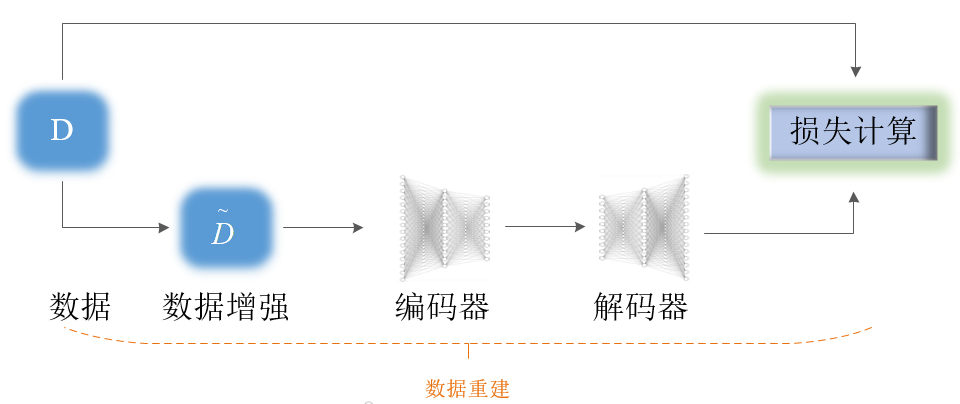
\includegraphics[width=0.8\textwidth]{self2.png}
	\caption{典型的生成型推荐算法示意图}
	\label{2Fig:self2}
\end{figure*}
%*******************************
生成型的推荐算法旨在通过使用扰动后的数据输入来重建原始输入,从而编码数据中的内在相关性。典型的生成型推荐算法如图~\ref{2Fig:self2}所示。根据它们的重建目标,可以将这些推荐算法分为两类:结构生成(Structure Generation)和特征生成(Feature Generation)。
\subsubsection{结构生成}
结构生成利用结构信息来监督模型,通过将基于屏蔽、随机丢点、随机丢边的增强操作应用于原始输入数据,可以得到其数据增强,然后训练模型对输入数据本身进行重建。例如,BERT4Rec\cite{sun2019bert4rec}通过将序列中的物品随机屏蔽,用特殊标记[mask]替换,然后重建交互下序列。最近的研究 \cite{geng2022recommendation,zhang:sigir} 迈出了探索提示学习和个性化结合的第一步。它将所有的推荐数据转换为自然语言序列,并在预训练期间使用掩码语言模型进预训练,并应用于推荐任务。
\subsubsection{特征生成}
特征生成利用特征信息来监督模型,通过在增强数据上学到的特征表示对原始特征表示进行重建。特征生成问题可以描述为一个回归问题,通常使用均方误差MSE描述重建特征表示和原始特征表示的距离。典型的方法如PMGT\cite{liu2021pre}。该方法使用提取的图像和文本特征初始化物品特征,并对采样节点的一部分进行屏蔽,然后训练基于Transformer的推荐模型,以重建恢复屏蔽节点的特征。对于序列特征生成,Ma等人\cite{ma2020disentangled}提出使用过去的行为来重建未来序列的特征表示。具体而言,将给定行为序列背后的意图进行分解,并在涉及共享意图的子序列之间进行重建。

生成型自监督推荐通常遵循掩码语言模型的流程,并依靠Transformer的强大能力取得较好的效果。特别最新的研究是将所有的推荐数据转换为自然语言序列,并在预训练期间使用语言建模目标进行预训练,但对计算资源要求较高。对于新闻推荐或通用表示的大规模数据集进行训练,则对计算资源提出了更高的要求。


\subsection{预测型推荐算法}
%*******************************
\begin{figure*}[h!]
	\centering
	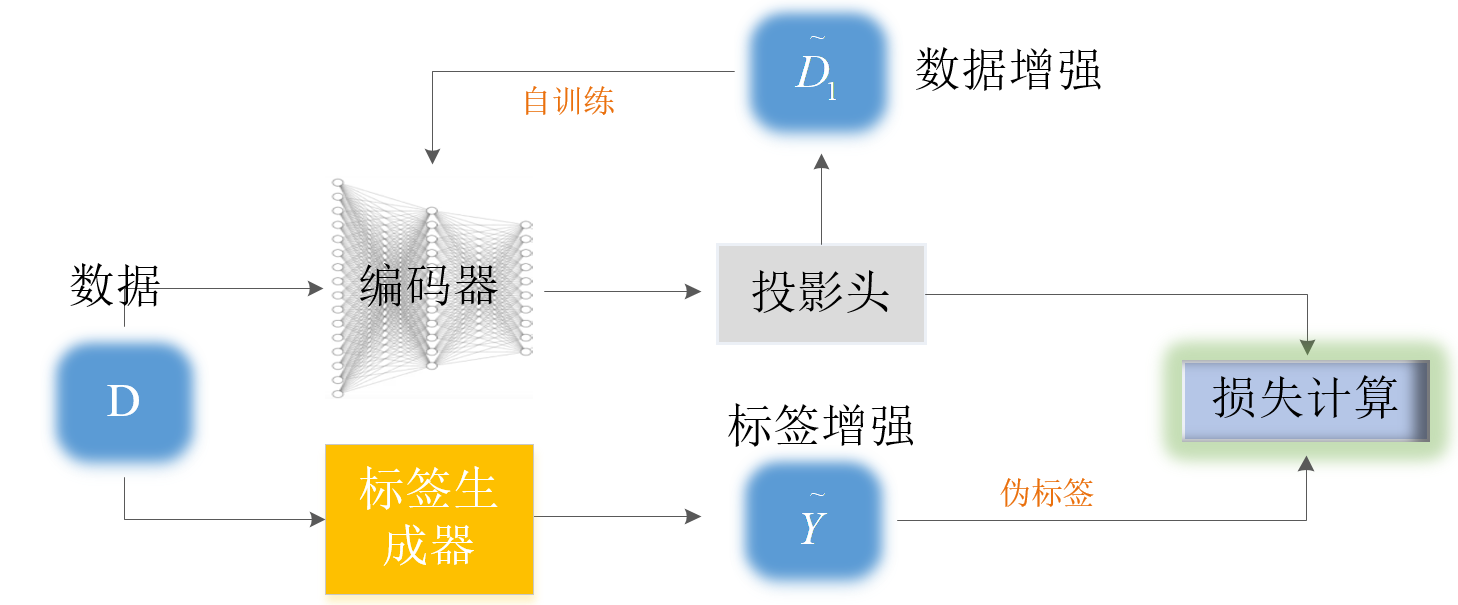
\includegraphics[width=0.8\textwidth]{self3.png}
	\caption{典型的预测型推荐算法示意图}
	\label{2Fig:self3}
\end{figure*}
%*******************************
预测型推荐算法和生成型推荐算法都涉及预测,但底层目标是不同的。生成型推荐算法侧重于预测原始数据中缺失的部分;而预测型推荐算法从原始数据中生成新的样本或标签以引导训练任务。典型的预测型推荐算法如图~\ref{2Fig:self3}所示。根据预测的任务,可以将预测型推荐分为两个分支:样本预测和伪标签预测。

\subsubsection{样本预测}
样本预测通常利用预训练模型生成的虚拟样本来监督模型,然后训练推荐模型对样本进行预测,这一方法广泛应用于序列推荐。例如,ASRep\cite{liu2021augmenting}首先以逆向方式预训练基于Transformer的编码器SASRec\cite{kang2018self},以使编码器能够生成虚拟样本。通过将虚拟的子序列添加到原始序列的开头,得到增强的序列。然后以从左到右的方式在增强的序列上进行微调,以预测原始序列中的下一个物品。例如,BiCAT\cite{jiang2021sequential}认为逆向增强可能与原始相关性不一致,于是提出同时从左到右和从右到左的方向预训练编码器,这种双向训练可以弥合逆向增强和正向推荐之间的语义差异。

\subsubsection{标签预测}
标签预测利用虚拟标签来监督模型,通过预训练的模型生成虚拟标签,然后训练推荐模型对虚拟标签进行预测。根据预测的标签形式,这些预测任务可以被形式化为关系预测和相似性预测。对于离散型标签,描述的通常是两个对象之间的关系,相应的预测任务是预测该关系是否存在。此类离散型的虚拟标签的预测任务可以被形式化为一个分类问题。例如,PTUM\cite{wu2020ptum}受BERT中的下一句预测(NSP)\cite{Devlin:2018:bert}启发,提出了预测两个序列之间的关系。该方法首先将用户行为序列分为两个不重叠的子序列,然后根据过去的交互序列预测候选物品是否为未来的交互序列。对于连续性标签的相似度预测任务,代表性的方法是BUIR\cite{lee2021bootstrapping}。该方法受到视觉模型BYOL\cite{BYOL:2020:NIPS}启发,采用了两个不对称的编码器(一个在线网络和一个目标网络)相互监督,其中目标网络生成了一个虚拟的相似度标签,用于监督在线网络的训练。

由于预测型推荐算法以动态的方式获取样本和伪标签,它们会随着模型参数不断演化,这样可以改进自监督信号,从而可能提高推荐性能。然而,大多数预测型推荐算法使用启发式方法获取伪标签,伪标签的可靠性、合理性以及与推荐任务的相关性尚缺乏评估。

%\subsection{混合型推荐算法}
%%*******************************
%\begin{figure*}[h!]
%	\centering
%	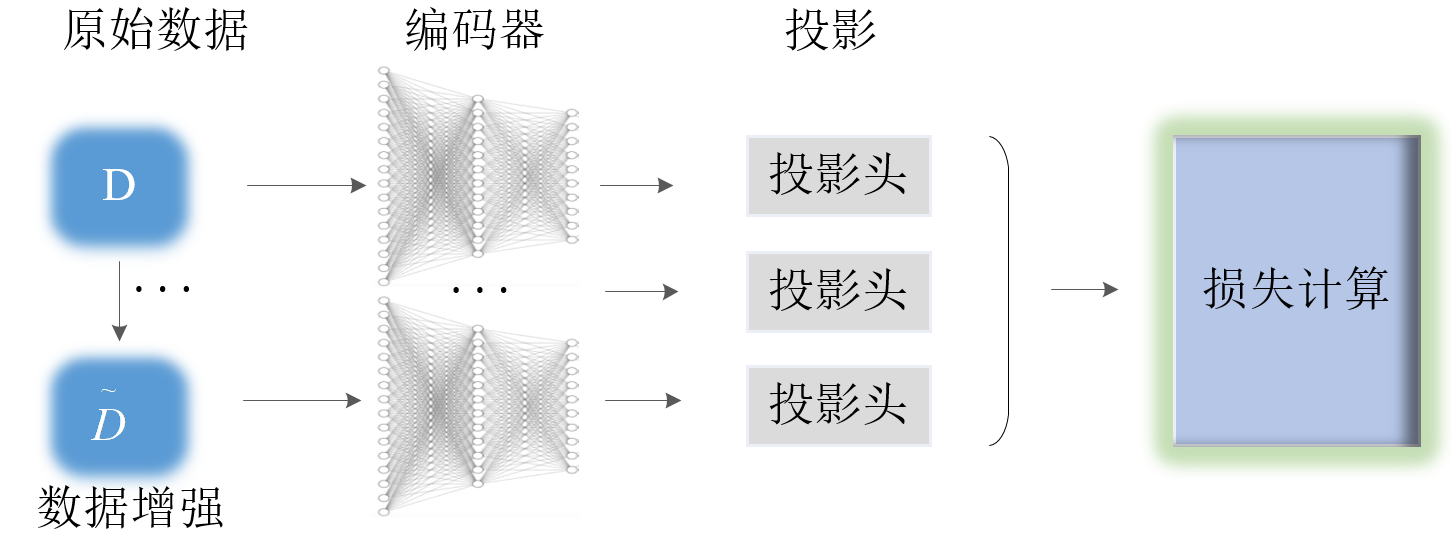
\includegraphics[width=0.9\textwidth]{self4.png}
%	\caption{典型的混合型推荐算法示意图}
%	\label{2Fig:self4}
%\end{figure*}
%%*******************************
比型推荐算法、生成型推荐算法和预测型推荐算法是自监督推荐的三种主要形式。混合方法\cite{bian2021contrastive,wang2023curriculum}利用不同的自监督信号,并组合多种类型的预训练任务,获得了增强和全面的自监督信号,在训练效果上比单一的自监督信号具有优势。然而,混合方法面临着协调多个自监督任务的问题,通常需要手动搜索超参数,以平衡不同的自监督任务。

%\textbf{协同自监督}使用多个自监督任务协同工作,以获取更全面的自监督信号。以CCL\cite{bian2021contrastive}为例,该方法提出了一种基于Transformer模型的预训练策略,将生成性预训练任务与对比性预训练任务进行组合。其中,生成性任务涉及到掩码物品的预测,预测的概率被用来增强序列,然后与原始序列进行对比。\textbf{并行自监督}方法的不同之处在于,多个自监督任务之间没有相关性,它们并行工作。以CHEST\cite{wang2023curriculum}为例,该模型组合了生成性和对比性任务。CHEST通过随机游走形成特定交互的子图。一方面,利用局部上下文信息在生成性任务中预测子图中的掩码节点/边。另一方面,利用全局相关性在对比任务中拉近原始子图和增强子图来学习子图级别的语义。

\section{对比学习相关工作}
对比学习在计算机视觉、自然语言处理等诸多领域取得了瞩目的成就,也是自监督推荐的主要实现形式\cite{SSR:2023:TKDE}。正样本、负样本以及对比损失是对比学习的核心组件,也是提升推荐性能的关键。本节首先介绍对比学习的概念,着重梳理推荐算法中广泛使用的BPR损失与InfoNCE的联系;然后梳理对比学习的相关工作,包括正样本增强、负样本采样、对比损失函数设计。
\subsection{对比学习基础概念}
从统计学习的角度来看,机器学习模型可以分为两类:生成模型和判别模型\cite{li:2019}。给定特征$X$和标签$Y$的联合分布$P(X,Y)$,生成模型旨在建模
\[p(X|Y=y)= \frac{p(X,Y)}{p(Y=y)}\]
而判别式模型旨在建模
\[p(Y|X=x)= \frac{p(X,Y)}{p(X=x)}\]
生成式模型需要重构特征$X$的像素级信息,从而捕捉特征之间的潜在关系。而判别式则是直接对后验概率建模,旨在激励编码器编码不同类别样本之间的差异特征,不编码像素级特征。对比学习属于判别式的一种,旨在通过噪声对比估计(Noise Contrastive Estimation, NCE)\cite{Gutmann:2010:ICAIS}的目标函数在比较中学习(Learn-to-Compare)
\begin{eqnarray}
\mathcal{L}_\textsc{Nce} = \mathbb E[-\log \frac{\exp(f(x)^Tf(x^+))}{\exp(f(x)^Tf(x^+))+\exp(f(x)^Tf(x^-))}]
\end{eqnarray}
其中,$x$是锚点,在推荐中通常选择用户$u$,$x^+$是锚点的正例,在推荐中通常选择为已交互的物品$i$;$x^-$为锚点的负例,在推荐中通常选择为未交互的物品$j$。$f$是编码器,$f(x)^Tf(x^+)$是由编码器参数化的正例对相似度预测得分,通常为内积相似度或者余弦相似度,记为$\hat{x}_{ui}$。类似地,$f(x)^Tf(x^-)$是负例对相似度预测得分,记为$\hat{x}_{uj}$。可以看到,NCE损失函数与BPR损失\cite{Steffen:2009:UAI}的联系:
\begin{eqnarray}
	\mathcal{L}_\textsc{Nce} 
	&=& \mathbb E[-\log\frac{\exp(\hat{x}_{ui})}{\exp(\hat{x}_{ui})+\exp(\hat{x}_{uj})}]\nonumber \\
	&=& \mathbb E[-\log\frac{1}{1+\exp(\hat{x}_{uj}-\hat{x}_{ui})}]\nonumber \\
	&=& \mathbb E[-\log \sigma (\hat{x}_{ui} - \hat{x}_{uj})]\nonumber \\
	&=& \mathcal{L}_\textsc{Bpr} 
\end{eqnarray}
其中$\sigma(\cdot)$为sigmoid函数。在实践中,由于要引入正则化项避免过拟合,而正则化项又等价于高斯分布先验密度的对数,从而BPR将上式解释为观测到的有序对的最大后验估计。尽管BPR和NCE有着不同的解释,但是BPR与NCE有着完全相同的数学形式,共享相同的优化目标。

需要说明的是,正例或者负例的语义是由自监督信号确定的。例如SimCLR\cite{Chen:2020:ICML}所使用的自监督信号是“图像增强的语义不变性”,从而把原图的增强定义为正例;BPR\cite{Steffen:2009:UAI}的自监督信号是“用户对已交互物品的偏好强于未交互物品”,从而将已交互物品定义为正例;LightGCL\cite{lightgcl:2023:ICLR}的自监督信号是“用户物品二分图(Graph)轻微扰动的语义不变性”,从而将相同的节点定义为正例。总而言之,具体的正例或负例语义由自监督信号决定,可以根据任务以及场景进行迁移和拓展。将NCE中加入更多的负例,那么可以得到InfoNCE损失\cite{Oord:2018:arxiv}:
\begin{eqnarray}
	\mathcal{L}_\textsc{InfoNCE} = \mathbb E[-\log \frac{\exp(f(u)^Tf(i))}{\exp(f(u)^Tf(i))+\sum_{n=1}^{N}\exp(f(u)^Tf(j_n))}]
\end{eqnarray}

可以看到,\textbf{NCE和BPR都是InfoNCE损失负例个数$N=1$的特例}。以最具一般性的InfoNCE损失为例,它的含义是正确分类正样本的交叉熵\cite{Oord:2018:arxiv},最小的InfoNCE损失为0,在正例相似度得分与负例相似度得分满足$f(u)^Tf(i)- f(u)^Tf(j_n)\rightarrow +\infty, n \in \{1,2,\cdots N\}$时取到。这一结论也适用于NCE和BPR,只是负例个数$N=1$。

进一步地,相似度分数与欧氏距离是一一对应的负相关关系。对于投影到单位超球面的两个$d$维向量$f(u) = (u_1,u_2,\cdots,u_d)$和$f(i) = (i_1,i_2,\cdots,i_d)$欧式距离$d(f(u),f(i))$与内积相似度分数$f(u)^Tf(i)$存在如下关系:
\begin{eqnarray}
d(f(u),f(i)) &=& \sqrt{(u_1-i_1)^2+\cdots +(u_d-i_d)^2} \nonumber \\
&=&\sqrt{2-2f(u)^Tf(i)} \nonumber
\end{eqnarray}
因此相似度分数越高,距离越近。成对损失或者对比损失与常用的均方误差损失具有明显的区别:均方误差损失是基于样本和监督标签计算得到;而成对损失或者对比损失是基于多个样本的特征表示计算得到,不涉及显式的监督标签。

基于上述分析,可以从三个方面归纳对比学习的特征:
\begin{enumerate}
\item 从数值角度看,对比学习优化正例得分大于负例得分,只优化相似度分数的差值,不优化具体值,以激励学习数据的内在结构和特性。
\item 从嵌入空间看,对比损失激励编码器拉近正例与锚点的距离,推远负例与锚点的距离,实现编码不同样本的差异特征,而非样本本身的像素级信息。文献\cite{Wang:2022:KDD}和文献\cite{Wang:2020:ICML}分别阐释了优化BPR损失以及InfoNCE损失都是渐进地优化正样本一致性(Alignment)、负样本的均匀性(Uniformity)\footnote{其中一致性要求正样本尽量接近,均匀性要求两个随机样本尽量分散。}。
\item 从统计角度看,对比学习优化“正确分类正样本的概率”\cite{Oord:2018:arxiv},体现判别式方法的特征,即直接对样本所属类别的后验概率建模。
\end{enumerate}

%\section{对比学习相关工作}
%对比学习有几个关键组件:(1)负例,(2)正例,(3)网络架构,(4)对比损失函数,共同决定了对比学习的效果。本节根据对比学习的组件,分别从负例采样方法、正例增强方法、网络架构设计和损失函数设计四个方面总结对比学习的相关工作。
\subsection{负样本采样方法相关工作}
%*******************************
\begin{figure*}[!]
	\centering
	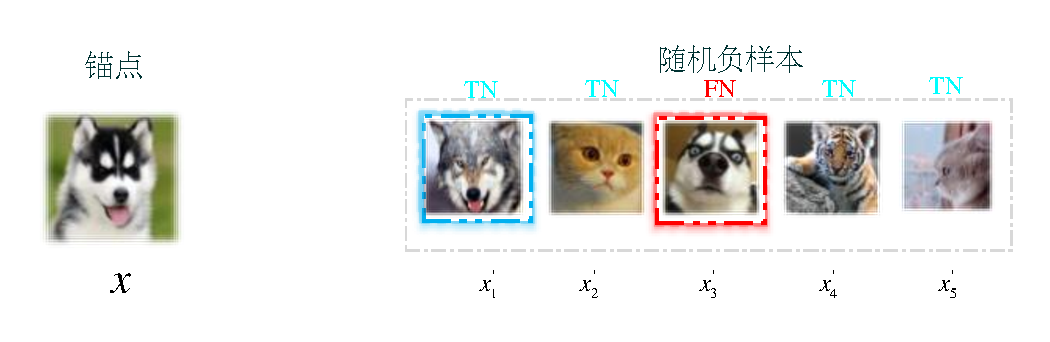
\includegraphics[width=0.9\textwidth]{fhn.pdf}
	\caption{困难负例和伪负例示意图}
	\label{2Fig:illustrative}
\end{figure*}
%*******************************
对比学习有两个关键目标,拉近正样本并推远负样本。如果仅仅拉近正样本,即只最小化正样本之间的距离,可能会使得神经网络学到坍缩的解,即为所有的样本输出相同的表示。因此,推远负样本也必不可少。但是在大多数情况下缺乏明确的负信号,因此从未标注样本中采样负例的负采样策略被广泛研究。以图\ref{2Fig:illustrative}的一个直观的示例解释负采样策略的两个关键目标:锚点为狗,样本$x_1^\prime$是狼,与锚点不同类,但是特征很相似,称为困难负样本(Hard Negative Sample)。样本$x_3^\prime$是狗,与锚点同类,由于缺乏监督标签也出现在负例候选集,称为伪负样本(False Negative Sample)。为了使得同类样本的表示距离较近,那么$x_1^\prime$狼这个困难负例应该被选作负样本,使其被推远,防止其混入狗这个类别;且$x_3^\prime$狗这个伪负例不应该被选作负样本,防止其被推远。推荐领域的任务也是一样,只是正负样本语义是喜欢与否。负采样(NS)的策略是从候选的未标注样本中采样负样本,核心目标围绕如何采样困难负样本且剔除伪负样本展开。许多研究表明,负采样对于提高下游的分类或推荐性能非常重要~\cite{Steffen:2014:WSDM,Zhang:2013:SIGIR,Ding:2020:NIPS,Park:2019:WWW,Huang:2021:KDD,Ding:2019:IJCAI,Yang:2020:KDD}。

\subsubsection{采样困难负样本}
采样困难负样本的主要目标是采样类似于样本$x_1^\prime$这样的困难负样本。它们与正例很相似,但是所属类别为负类。由于这两个样本在特征上相似度很高, 难以区分,在经过网络提取特征之后, 它们特征之间的相似度分数也比较高。采样此类样本一方面会使得不同类别的困难负样本被推远,迫使神经网络学习难以区分的样本之间的边界;另一方面,这类样本与锚点的相似度分数较高,梯度值较大,从而神经网络的参数更新更多,提高模型训练效率。基于上述动机,很多困难负采样(Hard Negative Sampling)方法被提出,这类方法普遍采用随模型训练动态调整的采样分布,以针对困难负例进行采样~\cite{Steffen:2014:WSDM,Zhang:2013:SIGIR,Ding:2020:NIPS,Park:2019:WWW,Huang:2021:KDD,Ding:2019:IJCAI}。

在推荐领域,困难负采样实现的典型思路是采样相似度分数较高,或排序位置靠前的样本。最具代表性的困难负采样方法为动态负采样\cite{Zhang:2013:SIGIR}。动态负采样通过在若干个候选的负例中采样相似度分数比较高的样本,从而实现每个样本的采样概率正比于其相对排序位置。类似地,Steffen等人\cite{Steffen:2014:WSDM}提出针对排名位置靠前的样本进行采样。这两个经典思想是类似的,因为排序位置与相似度分数是一一对应的。除了使用分数相似度或者相对排序位置来表征样本的困难等级(Hardness Level),还有研究者使用图的相关信息来采样困难负样本。例如,Wang等人~\cite{Wang:2020:WWW}和Wang等人~\cite{Wang:2021:CIKM}提出利用知识图谱上的关系类型来采样困难负例。另一种方使用较多的是选择与正例在图结构上相似的困难样本~\cite{Chen:2019:WWW,Wang:2021:TKDE,Ying:2018:KDD}。文献\cite{shi2023theories}分析了,困难负采样实际上是在优化推荐列表指定伪正例例率(FPR)范围内的AUC面积(One-way Partial AUC, OPAUC),但没有考虑伪负例问题。

\subsubsection{剔除伪负样本}
剔除伪负样本的主要目标是避免采样类似于样本$x_3^\prime$这样与锚点同类的样本。由于缺乏标签,它们虽然出现在负例候选集,但是所属类别为正类。在推荐领域,这类样本对应于用户没有看到过,但是潜在喜欢的物品。由于这个样本所属类别为正类,因此应当避免采样到此类样本,防止其在嵌入空间被推远。另一方面,采样此类物品,会使得模型误判用户的兴趣边界。因此,负采样的另外一个重要目标就是防止采样到伪负例。最普遍方法是使用附加信息来避免采样伪负例。这些附加信息对于提取负信号非常直观,例如社交网络中用户的连接关系~\cite{Zhao:2014:CIKM,Wang:2016:CIKM}、用户的地理位置~\cite{Yuan:2016:IJCAI,Liu:2019:IJCAI},以及额外的交互数据,如已查看但未点击的数据~\cite{Jingtao:2019:IJCAI, Jingtao:2018:WWW},但是这些额外信息通常不好获得,只有特定的数据集才有。

为了避免采样伪负例,还有一类新的方法是使用多个未标记样本中生成虚拟的负样本用于模型训练。例如,Huang等人~\cite{Huang:2021:KDD}提出通过混合候选负样本的嵌入来合成虚拟的困难负例。Jun等人~\cite{Jun:2017:SIGIR}和Park等人~\cite{Park:2019:WWW}设计了生成对抗神经网络来生成虚拟的困难负例。合成虚拟负样本的方法也广泛使用在计算机视觉中,例如Zhu等人\cite{zhu:2021:iccv}提出了在特征空间上将负样本对应的嵌入插值,类似于构造了虚拟的负样本,而对正样本的嵌入外推,最终提高了对比学习的效果。 Zhong 等\cite{zhong:2021:cvpr}提出了一种结合图像混合 (Mixup) 技术的困难样本构造方法, 首先使用Mixup合成虚拟的负样本,然后依据合成负样本的相似度分数选择困难的合成负样本进行对比学习训练。

总体来说,负采样方法取得较大进展,特别是困难负采样方法对于下游任务性能提升效果非常显著。采样困难样本是容易实现的,只需要采样相似度分数高或者距离近的样本。但是如何从困难样本中采样真负例,还是严重依赖额外信息作为监督信号。尽管合成虚拟负样本的方法看似避免了采样伪负例,但是它的实质是将更多的样本包含在对比损失的分母中:虚拟样本嵌入是若干个负例的混合,那么虚拟样本的相似度分数是这几个负例相似度分数的函数,更多的样本用于合成虚拟样本,导致更多的样本包含在对比损失的分母中,并没有从根本上解决伪负样本问题。
\subsection{正样本数据增强相关工作}
正样本数据增强的目标是获取语义不变的正样本用于对比。数据增强是获取语义不变的正样本的主要途径,也是提升自监督信号的重要来源。在计算机视觉中,通常的做法是通过在锚点$x$上进行某些语义不变的数据增强来获得正样本$x^+$,如随机裁剪和翻转\cite{Oord:2018:arxiv},图像旋转\cite{Komodakis:2018:ICLR},和颜色失真\cite{Szegedy:2015:CVPR}等。然而,仅采用单一的图像增强方法并不利于性能提升,SimCLR\cite{Chen:2020:ICML}方法综合比较了一系列图像变换方法的效果,并发现将随机裁剪和颜色失真组合起来的变换方式能够获得更好的效果。

受到图像领域的启发,在推荐领域的数据增强工作也得到了广泛的研究。然而,推荐系统数据集通常以用户物品二分图的形式存在,节点只包含ID,往往使用基于图的策略进行增强。在推荐中数据增强的核心思想是在原有用户二分图结构的基础上略作扰动。这种增强的用户物品二分图被认为保留了结构信息,相同ID的节点即为正样本。图数据的增强策略可以分为以下几种(1)基于特征的增强\cite{liu2022local,velivckovic2018deep,zhu2020deep,you2020graph,pmlr-v139-you21a}:仅对节点或者边的特征矩阵进行变换。通常随机屏蔽节点或边属性的一小部分,并用常数或随机值替换。(2)基于结构的增强\cite{pmlr-v119-zheng20d,10.1145/3437963.3441734,10.1145/3437963.3441720,page1998pagerank}:仅对邻接矩阵进行变换。通常随机(或手动)在图中添加或删除一小部分边,包括边扰动\cite{pmlr-v119-zheng20d,10.1145/3437963.3441734}、节点插入\cite{10.1145/3437963.3441720}和边扩散\cite{page1998pagerank}、图采样\cite{pmlr-v119-zheng20d}等方法。

%(3)基于标签的增强\cite{Steffen:2014:WSDM,zhang2020graph,verma2019manifold}:由于图上人工标注标签的不足,通过标签增强用于增加有限的标记训练数据。它可以分为两类:一类是伪标签的增强,例如PTUM\cite{wu2020ptum}将用户行为序列分为两个不重叠的子序列,构建了两个序列之间的关系的标签。第二类是数据混合\cite{zhang2020graph,verma2019manifold},直接插值构建虚拟的负样本。VGCL\cite{yang2023generative}综合考虑了特征增强和结构增强的缺陷,利用变分图重构来估计每个节点的高斯分布,然后从估计分布中进行多个采样来,生成多个对比视图。LightGCL\cite{lightgcl:2023:ICLR}则将归一化的邻接矩阵进行奇异值分解,通过抛弃被认为是噪声的较小奇异值,获得了增强视角的图用于对比。

总体来说,由于图数据具有固有的非欧几里得特性,很难将图像中的随机剪裁、反转、颜色失真等保持语义不变的数据增强方法应用于图数据。基于随机过程的图数据增强可能会损失图中重要的结构信息,因为随机丢弃的点或者边可能会体现图的重要结构信息。此外,图增强对于推荐任务的有效性存在一些质疑\cite{yu2022graph},有待更深入和更系统地调查。

%
%\subsection{网络架构设计的相关工作}
%既然数据增强对于提升自监督对比学习的效果至关重要,那如设计更有效的网络架构,从而享受更密集的数据增强带来的好处?此外,负例的未标注是自监督对比学习与有监督对比学习的主要差异。既然有限的监督信号下难以避免采样伪负例。那么是否可以不用负样本,同时避免神经网络学到坍缩解?基上述两个主要动机,不同的网络架构被提出。由于相似度分数$\exp(f(x_1)^T,f(x_2))$计算涉及两次对样本的编码,下文把编码第一个样本的网络称为网络分支1,把编码第二个样本的网络称为网络分支2。根据两个网络分支的架构是否相同,可以分为同构网络和异构网络:前者网络分支架构相同,后者网络分支架构不同;根据两个网络分支参数的更新方式是否相同,可以分为同步网络和异步网络:前者通常采用端到端的反向传播方式更新网络参数,后者的网络分支更新方式不同,往往分别使用梯度法和动量法分别跟新两个网络分支参数。
%\subsubsection{同步同构网络架构}
%典型的同步同构网络如图\ref{2Fig:arc1}所示,代表性工作是SimCLR\cite{Chen:2020:ICML}。它采取了最自然的端到端地反向传播的方式更新神经网络参数,且两个网络分支的架构完全相同。给定一个样本,经过两次增广获得正样本对,从而受益于更密集的数据增强;然后, 通过同一个神经网络模型将样本投影到嵌入空间。这里,同一个神经网络模型即可以看作两个同构的网络分支。 对同一个Mini Batch的$N$个数据进行同样操作后,得到$2N$个表示向量;然后, 根据这$2N$个表示向量经过多层感知机(MLP)非线性映射得到投影;最后,根据投影计算InfoNCE损失,然后反向传播更新梯度。由于它使用一个神经网络模型,可以看作两个完全相同的网络分支,因此是同构网络;此外,两个网络分支是端到端地进行反向传播更新参数,因此是同步网络。
%%*******************************
%\begin{figure*}[h!]
%	\centering
%	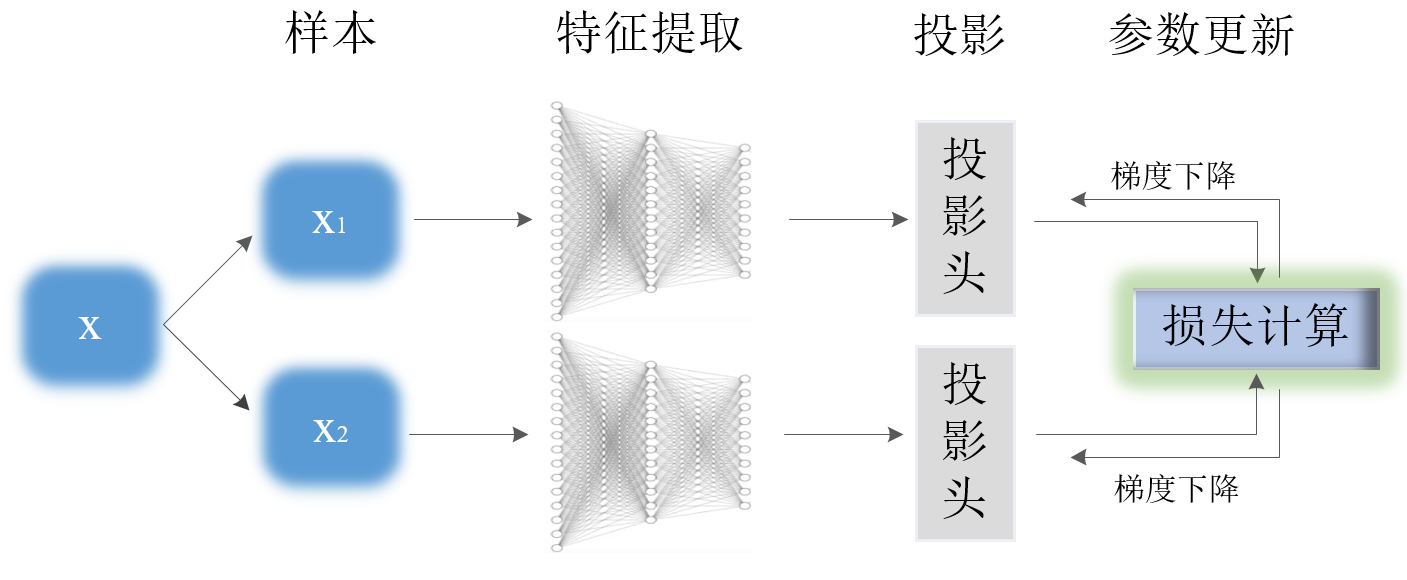
\includegraphics[width=0.8\textwidth]{arc1.png}
%	\caption{同步同构网络架构示意图}
%	\label{2Fig:arc1}
%\end{figure*}
%%*******************************
%
%在推荐中的网络架构大都可以归纳为同步同构网络架构,但工作机制略有不同。以最常用的LightGCN\cite{Xiangnan:2020:SIGIR}为代表,第一个网络分支编码用户表示,第二个网络分支编码物品表示,即双塔结构。聚合后的用户物品表示无需投影,直接计算损失,然后反向传播更新用户和物品表示。由于用户物品表示都是采用梯度更新的方式,因此是同步更新方式;此外用于聚合用户和物品的图卷积神经网络结构相同,因此是同构网络。另一种具有代表性的是LightGCL\cite{lightgcl:2023:ICLR}:第一个网络分支编码原图的用户表示,第二个网络分支依旧编码增强图的用户表示。LightGCN优化用户和喜欢的物品表示尽量相似,和不喜欢的物品表示尽量不相似;LightGCL则优化不同视图下同一个用户的表示尽量相同,与其他用户表示尽量不同,物品表示同理。这种差异主要是源自于对正负样本的定义和语义不同:LightGCN中用户和喜欢的物品构成正样本对,LightGCL中不同视图下的同一用户构成正样本对,同一物品也构成正样本对。这是正例对(或者负例对)的定义和语义不同,不影响网络架构的组织形式以及参数更新方式。
%\subsubsection{同步异构网络架构}
%%*******************************
%\begin{figure*}[h!]
%	\centering
%	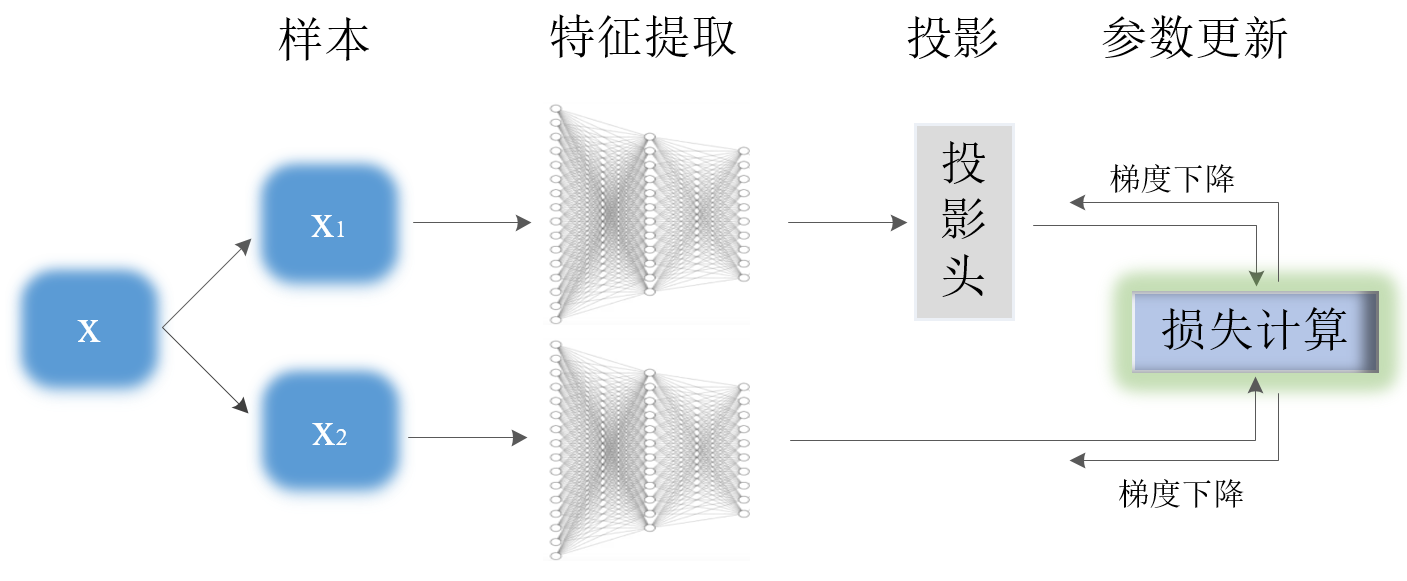
\includegraphics[width=0.8\textwidth]{arc2.png}
%	\caption{同步异构网络架构示意图}
%	\label{2Fig:arc2}
%\end{figure*}
%%*******************************
%典型的同步异构网络如图\ref{2Fig:arc2}所示:两个网络分支的参数更新方式是相同的,都采用梯度下降更新参数;但网络分支的架构不同,两个网络分支采用不同的网络结构。网络结构的不同主要有三种:(1)分支1包含投影头,分支2不包含投影头\cite{Oord:2018:arxiv}。(2)分支1和分支2都含有投影头,但投影头的结构不相同\cite{misra:2020:CVPR}。(3)用于特征提的分支1和分支2的网络结构不相同\cite{chaitanya:2020:NIPS}。以第一种为例,介绍同步异构网络架构的工作机制,典型的工作是对比预测编码(contrastive predictive coding, CPC)。在该方法中,分支1接收某个时间点的数据作为输入,分支2接收未来某个时间点的数据作为输入,目标是利用分支1的输出来预测分支2的输出,以最大化已知数据和待预测数据的互信息。在计算损失后,两个网络分支均按梯度法更新参数。
%\subsubsection{异步同构网络架构}
%%*******************************
%\begin{figure*}[h!]
%	\centering
%	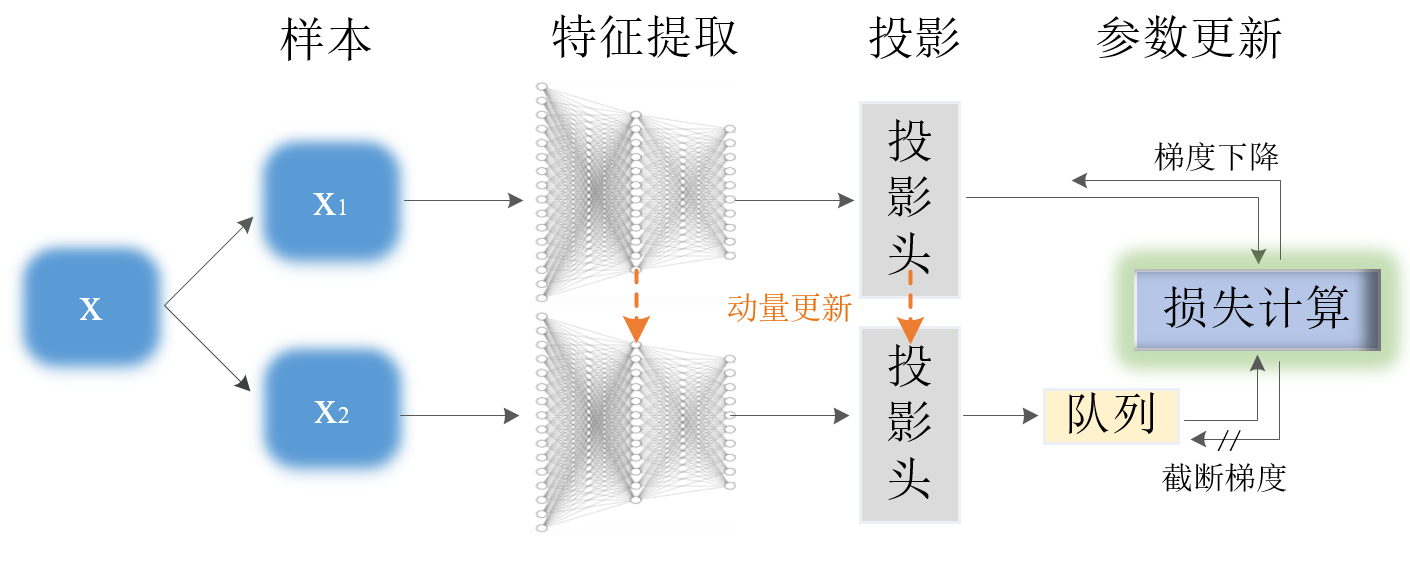
\includegraphics[width=0.8\textwidth]{arc3.png}
%	\caption{异步同构网络架构示意图}
%	\label{2Fig:arc3}
%\end{figure*}
%%*******************************
%典型的异步同构网络架构如图\ref{2Fig:arc3}所示:两个网络分支架构相同,但参数更新方式不同:网络分支1采用梯度下降更新参数,而网络分支二采用动量法更新参数。使用这种异步同构的网络架构典型工作是MoCo\cite{He:2020:CVPR}。网络分支1和网络分支2架构完全相同,初始化参数也相同。第一个网络分支按照正常操作获得样本投影的特征,但是第二个网络分支把投影的特征压入队列,直到队列达到指定长度以后,对最先入队的样本特征执行出队操作,从而获得一个较大的负样本数量。最后,根据正样本的投影特征计算损失。回传梯度时,只有第一个网络分支执行反向传播更新参数,第二个网络分支的参数根据第一个网络学到的参数进行动量更新。记第一个网络分支的参数为$\theta$,第二个网络分支的参数为$\xi$,那么它们的更新方式可以写为:
%\begin{eqnarray}
%	\theta &\leftarrow& \text{optimizer}(\theta,\nabla_\theta \mathcal{L}) \nonumber\\
%	\xi &\leftarrow& \tau \xi + (1-\tau)\theta \nonumber
%\end{eqnarray}
%其中第一个网络分支的参数$\theta$通过梯度法更新以后,将学到的最新的参数$\theta$,取$(1-\tau)\theta$用于更新第二个网络分支的参数。可以看到,只有第一个网络分支参数更新以后,才能更新第二个网络分支,因此称这种参数更新方式为异步法。当衰减系数$\tau$比较大时,第二个网络分支的参数更新幅度很小。异步法区别于端到端地使用梯度下降法更新两个网络分支,它们的更新是同步的。
%
%MoCo的第一个核心操作是对网络分支2编码得到的特征执行入队操作,解耦了负样本数量与批量大小,负样本数量不再受限于GPU显存大小,从而可以为对比学习设定一个较大的负样本数量。而较大的负样本数量会推高已知数据和待预测数据互信息的下界,从而取得更好的性能。此外,较大的负样本数量也会使得正例的梯度值增加,使得神经网络模型从正样本的数据增强中学到更多信息。MoCo的第二个核心操作是,网络分支2根据网络分支1学到的最新参数,使用动量法跟新参数而非使用梯度法更新参数,一方面可以避免伪负例产生的错误梯度的影响,另一方面避免神经网络学到坍缩的解。
%
%\subsubsection{异步异构网络架构}
%
%典型的异步异构网络架构如图\ref{2Fig:arc4}所示:两个网络分支架构不同,参数更新方式也不同,代表性工作是BYOL\cite{BYOL:2020:NIPS}。在参数更新方式上,网络分支1(在线网络)采用梯度下降更新参数,而网络分支2(目标网络)采用动量法更新参数。在网络结构设计上,两个网络分支采用MoCo作为主干网络,但投影头的数量不一致,网络分支1增加了一个预测头,以提高灵活性。在损失计算上,与先前的工作截然不同:之前的工作都涉及到同一批次内的其它样本作为负样本以计算对比损失,但是BYOL的计算只涉及一个样本的两个增强视角的特征投影,只约束正例对提取到的特征尽量相似。相当于完全抛弃了负例,只优化正例的对齐,不优化负例均匀,同时实现避免了神经网络学到了坍缩解。
%%*******************************
%\begin{figure*}[h!]
%	\centering
%	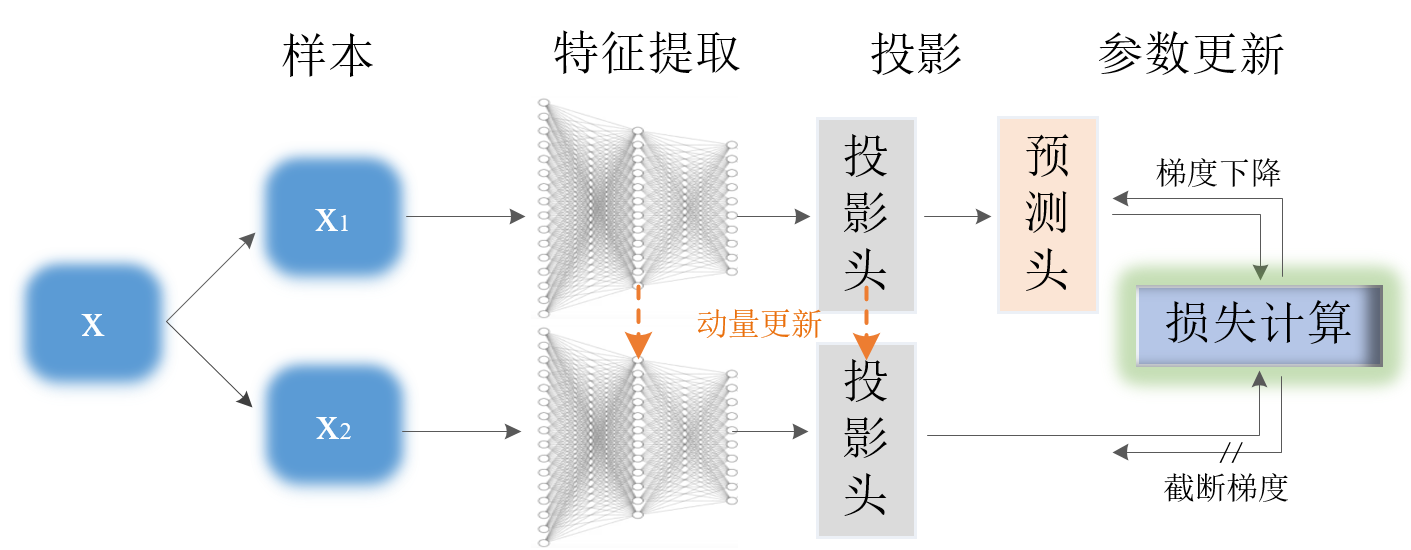
\includegraphics[width=0.8\textwidth]{arc4.png}
%	\caption{异步异构网络架构示意图}
%	\label{2Fig:arc4}
%\end{figure*}
%%*******************************
%
%BYOL的第一个核心操作是和MOCO一样,在线网络分支使用梯度法更新参数,第目标网络分支采用动量法更新参数。动量法更新也称指数滑动平均法(exponential moving average,EMA),尤其是在其衰减系数$\tau$比较大时,目标网络的参数更新很慢。第二个核心操作是给在线网络加了一个经过归一化的预测头,且其参数不会更新给目标网络,相当于在线网络提取的特征和目标网络提取的特征存在缓冲地带。这两个操作都有助于分散特征,避免神经网络学到坍缩解。第三个核心操作是损失的计算,完全不涉及负样本,只涉及正样本对的特征。具体的,是经过L2归一化的两个正样本对特征向量的均方误差,相当于只约束正样本对特征的方向。由于BOYL只优化正例对的均匀,不优化负例的均匀,从而避免了伪负样本的错误梯度问题。

\subsection{损失函数设计的相关工作}
损失函数是实现对比学习“拉近同类正样本、推远不同类负样本”的关键,从而激励编码器编码不同类别样本之间的差异信息,而非样本的像素级信息,是对比学习的核心组件。对比损失中应用最为广泛的是InfoNCE\cite{Oord:2018:arxiv},尽管BPR\cite{Steffen:2009:UAI}、NCE\cite{Gutmann:2010:ICAIS}是InfoNCE损失负例个数为1的特例,且工作远早于InfoNCE,但是InfoNCE率先构建了对比损失优化与互信息优化之间的关联。InfoNCE也广泛应用于推荐领域的图对比任务和偏好对比任务,文献\cite{Jiancan:2022:arxiv}证明了在偏好对比任务中,优化InfoNCE损失等价于优化NCDG指标。本节以更具一般性的InfoNCE损失为主线,梳理损失函数设计的相关工作。这些针对InfoNCE的改进可以很容易类比到负例个数为1的BPR损失。
\subsubsection{面向正负样本语义拓展的损失函数改进}
为了获取更密集的数据增强,SimCLR\cite{Chen:2020:ICML}将同一个样本增强两次,那么同一个批次内的N个样本经过两次数据增强就得到了2N个样本。同一个样本的两次增强$z_i,z_j$互为正例对,构造了如下对比损失
\[
\mathcal{L} = -\log \frac{\exp(f(z_i)^Tf(z_j))}{\sum_{k=1}^{2N}\mathbb I (k \neq i)\exp(f(z_i)^Tf(z_k))}
\]
其中分子是同一个样本的两个增强视图的相似度,分母是同一个样本的两个增强视图的相似度加上与其它图像两个增强视图的相似度,合计2N-1项。可以看到与InfoNCE的数学形式是一致的,只是拓宽了正负样本对的概念。MOCO\cite{He:2020:CVPR}变化在于负样本是一个提取的特征组成的队列,损失的计算方式与InfoNCE相同。

在推荐中通过一些附属信息将正负样本对的概念进行拓展,构造了更具细粒度的正负样本对,从而提取更密集的自监督信号。例如被购买的物品比只浏览的物品更受用户喜欢\cite{Qiu:2018:IS};多次交互的物品比只有一次交互的物品更受喜欢\cite{Lerche:2014:RS};用户未看到的物品应该比曝光给用户但没有交互的物品更受喜欢\cite{Wenhui:2019:WWW,Yu:2018:CIKM,Bin:2020:IS}。这类正负样本的语义下的对比学习任务是排序导向,目标是将用户喜欢的物品排在不喜欢的物品之前,与推荐任务具有一致性;此外,LightGCL\cite{lightgcl:2023:ICLR}将不同视图下的相同节点视为正样本对,不同节点视为负样本对。这类正负样本的语义对应的对比学习任务是学习图结构信息,与推荐任务不一致,通常要与第一类学习任务联合训练。在损失函数分析中,通常不区分由于正负样本对的概念拓展造成的损失函数与原始对比损失函数的差异。

\subsubsection{面向模型坍塌问题的损失函数改进}
由于对比损失优化正例对齐,神经网络的参数空间存在一种可能的解,它为所任意样本映射为同一个相同的特征表示,这样的解也称坍缩解或者模型坍塌\cite{jing2021understanding}。尽管负例参与学习训练有助于分散特征(Scatter Feature),避免模型坍塌,但也不能完全避免这种情况。基于这种情况DirectCLR\cite{jing2021understanding}取特征向量的前d维的子向量,计算对比损失
\[
\mathcal{L} = -\log \frac{\exp(f(z_i^\prime)^Tf(z_j^\prime))}{\sum_{k=1}^{2N}\mathbb I (k \neq i)\exp(f(z_i^\prime)^Tf(z_k^\prime))}
\]
其中,$z^\prime = z[0:d]$是原始特征向量的前d个维度构成子向量,这个对比损失与SimCLR损失的唯一区别就是只取每个特征向量的前d维。

BYOL\cite{BYOL:2020:NIPS}进一步改进了对比损失。对同一个样本的两次增强,两个网络分支学到的归一化特征表示分别记为$\bar q(z)$和$\bar z\prime $,BYOL优化归一化特征表示的均方误差:
\[||\bar q(z)-\bar z\prime||^2 =2-2\cdot \frac{\langle q(z),z\prime \rangle}{||q(z)||_2\cdot||z\prime||_2  } = 2-2\cos(q(z),z\prime)\]
其中为$q(z),z\prime$分别为两个网络分支学到的特征表示向量(未归一化)。可以看到,BYOL实际上只约束两个网络分支学到的特征表示的方向一致,并不规定正例对表示向量的具体模值。除了损失函数外,BYOL还通过精致的网络架构设计和正则化技术分散特征,避免神经网络学到坍缩解。

\subsubsection{面向梯度消失问题的损失函数改进}
InfoNCE损失函数的形式决定了其正例梯度等于所有负例梯度的和,符号相反\cite{Feng:2021:CVPR}。对于一个分数较小的负样本(容易负样本),或者分数较大的正样本(容易正样本),梯度容易消失,使得模型从样本中学到较少的信息。具体到负例个数为1的BPR损失中,就有正例的梯度等于负例的梯度,同样符号相反,使得梯度消失的问题更加明显,因此往往需要通过保持较大的负例个数N,以避免梯度消失的问题\cite{He:2020:CVPR}。于是解耦对比损失\cite{yeh:2022:ECCV}(Decoupled Contrastive Learning)去掉了InfoNCE失函数分母中两个正样本对之间的相似度,损失函数的形式计算如下:
\[
\mathcal{L} = -\log \frac{\exp(f(x)^Tf(x^+))}{\sum_{i=1}^{N}\exp(f(x)^Tf(x^-))}
\]
解耦对比损失避免了负样本数量对梯度的放缩,在一定程度上解决了容易正样本和容易负样本所导致的梯度消失问题。


\subsubsection{面向优化目标偏离问题的损失函数改进}
在自监督场景下,InfoNCE损失实际上优化实例之间的对齐和均匀,而非不同类别样本的均匀与对齐。更具体地,在自监督场景下,由于未标记的样本都被视作负样本,InfoNCE实际上是拉近正例与锚点之间的距离,\textit{推远任意样本与锚点之间的距离,而非负例与锚点之间的距离}。在个性化推荐中,任意未交互(未标注)的物品都被视作负例被推远;在计算机视觉中,锚点以外的任意未标记样本都被视作负例被推远。负例的无监督,使得自监督场景下InfoNCE偏离了原始的优化目标,对下游分泛化性能产生了不利的影响。为了鼓励编码器去编码数据的语义结构,拉近同类样本,推远不同类样本,ProtoNCE\cite{Li:2021:ICLR}通过改进正负样本对的语义,以改进对比损失。具体地,当前样本的特征与其对应的聚类中心构成正样本对,而与其他聚类中心形成负样本对,从而得到如下优化目标:
\[
\mathcal{L} = -\log \frac{\exp(f(x)^Tf(c_i))}{\sum_{i=1}^{C}\exp(f(x)^Tf(c_i))}
\]
其中$c_i$为聚类中心,也被称为原型(prototypes),通过在EM算法的期望步骤中执行k-means聚类得到。通过将正样本修改为锚点所属类中心,负样本修改为其他聚类中心,实现将优化目标改进为拉近样本与所属类别中心的距离,推远样本与其它类别中心的距离。这一思想在个性化推荐中也有应用\cite{lin2022improving}。

上述方案需要迭代计算,开销较大。另外一个解决负例无监督的途径是通过校正负样本相似度分数,以获取一个与有监督对比损失一致的改进损失函数,从而取得类似于监督学习的泛化效果,代表工作是去偏对比学习\cite{Chuang:2020:NIPS}(Debiased Contrastive Learning, DCL)。其核心思想是,由于伪负例包含在InfoNCE的分母中,导致的结果是分母中的负例相似度分数计算不准确。可以通过修正负例的相似度分数,实现对有监督对比损失的近似。其损失函数计算如下
\[
\mathcal{L} = -\log \frac{\exp(f(x)^Tf(x^+))}{\exp(f(x)^Tf(x^+) + N\cdot g}
\]
其中$g$是对真负样本与锚点相似度分数期望值的估计,其具体形式在后面的章节中会有更详尽的介绍。

在去偏对比学习\cite{Chuang:2020:NIPS}的伪负例去偏的基础上,HCL\cite{Robinson:2021:ICLR}进一步地考虑了硬负例挖掘,即将困难负样本推远离锚点。它遵循DCL的框架,并通过如下方式进一步地加权未标注样本的相似度分数:
\[\omega_i^\textsc{Hcl} = \frac{\hat{x}_j^\beta}{\frac{1}{N} \sum_{j=1}^{N}\hat{x}_j^\beta}
\]
其中$\hat{x}$是未标注样本与锚点的相似度分数,$\beta$是超参数。因此,未标注样本的相似度分数越高,其分配到的权重就越大,导致其被推的越远。基于估计校正的损失函数改进,避免了额外的计算开销,取得了很好的效果。

总体来说,损失函数设计相关工作取得较大进展,特别是在原理层面,现有的研究揭示了对比学习取得良好泛化性能的关键是(1)正样本特征的一致性;(2)负样本特征分布具有均匀性\cite{Wang:2020:ICML,Arora:2019:ICML}。从一致性要求考虑,应当防止同类样本被推远;从均匀性要求考虑,应当使得不同类样本被推远。对于一个未标注样本,无法确它所属类别,使得一致性和均匀性存在矛盾。尽管现有的去偏差方法通过损失校正构建了与有监督对比损失的关联,但是自监督对比学习与有监督对比学习仍存在较大距离,一致性与均匀性困境仍是一个尚待解决的问题\cite{Feng:2021:CVPR,zhang:cl}。

\section{预备知识}
本节介绍三个本文会频繁使用的工具,分别为经验分布函数、次序统计量和极大似然估计。
对于深度神经网络而言,准确推导其输出的相似度分数的分布是很困难的,本文会频繁使用来自样本计算得到的经验分布函数来刻画总体分布特征。此外,个性化推荐是一个排序任务,因此会频繁使用到次序统计量用于排序分析。最后,成对学习是极大似然估计量,因此也会频繁使用到。


\subsection{经验分布函数}\label{ecdf}
在介绍经验分布函数之前,先回顾累积分布函数(Cumulative Distribution Function, CDF)的定义。对于一个实值随机变量$X$,累积分布函数(CDF)在x处的值表示随机变量X取值小于或等于x的概率
\[F(x) = \mathbb P (X\leq x)\]
$F(x)$满足${\displaystyle \lim _{x\rightarrow -\infty }F(x)=0}$且${\displaystyle \lim _{x\rightarrow \infty }F(x)=1}$。

对于连续随机变量$X$,其累积分布函数CDF可以表示为其概率密度函数$f_X$的积分,如下所示:
\[{\displaystyle F(x)=\int _{-\infty }^{x}f_{X}(t)\,dt}\]
因此,只要给出概率密度函数$f_X(x)$的表达式,就可以准确计算累积分布函数$F(x)$。然而在绝大部分场景下,获取概率密度函数$f_X(x)$的表达式是困难的,那么累积分布函数$F(x)$的计算通常依赖于经验分布函数。

经验分布函数,通常也称为经验累积分布函数(empirical Cumulative Distribution Function, eCDF)是与样本的经验观测相关联的分布函数。在观测变量的任何指定值处,经验分布函数定义为小于或等于指定值的观测变量的比例:
\begin{eqnarray}
\hat F(x) = \frac{1}{N}\sum_{i=1}^{N} \mathbb I (X_i\leq x)
\end{eqnarray}
其中,$\mathbb I(\cdot)$是指示函数。以一个例子说明经验分布函数的计算。假设有五个独立同分布的观测值$\{3,7,2,6,4\}$,那么可以计算得到 $\hat F(1) = 0$,表明五个观测值小于等于1的占比为0;$\hat F(2) = 1/5$,表明五个观测值小于等于2的占比为1/5;$\hat F(3) = 2/5$,表明五个观测值小于等于3的占比为2/5。以此类推,$\hat F(100) = 1$,表明五个观测值小于等于100的占比为1。


经验分布函数$\hat F(x)$是标准的累积分布函数$ F_{X}(x)$的估计\cite{mou:2006}。对于固定的$x$,指示函数${\displaystyle \mathbb {I}({X_{i}\leq x})}$是一个参数为$p=F(x)$的伯努利随机变量。因此,${\displaystyle n{\widehat {F}}(t)}$是一个具有均值$nF(t)$和方差$nF(t)(1-F(t))$的随机变量。这意味着$\hat F(t)$是$F(t)$的无偏估计量。此外,根据Glivenko定理~\cite{glivenko:1933}证明了,经验分布函数一致收敛于分布函数。

在很多场景下,想获取累计分布函数(CDF)$F(x)$的解析表达式是非常困难的,但是计算经验分布函数(eCDF)却非常容易实现。于是可以通过计算经验分布函数(eCDF),以实现对抽象的分布函数的近似。经验分布函数是一个强有力的工具,通过少数观测样本对难以获取的分布函数进行近似,实现对总体分布特征的刻画,本文会多次使用这个工具。

\subsection{次序统计量}\label{order}
对于n个独立同分布随机变量$X_1, X_2, \cdots, X_n$,根据其取值升序排列,有
\[X_{(1)} \leq X_{(2)} \leq \cdots \leq X_{(n)} \]
那么称$X_{(k)}$为排序第$k$的次序统计量\cite{David:2004}。下面简单分析如何求解次序统计量$X_{(k)}$的概率密度表达式。

记随机变量$X$的概率密度为$f(x)$,相应的累积分布函数记为$F(x) = \int_{ - \infty }^x f(t)dt$,可以使用概率微元法\cite{mou:2006}求得次序统计量$X_{(k)}$的概率密度表达式。

对于随机变量的$n$个观测值$\{x_i\}_{i=1}^n$,一定存在一个足够小的区间$dx_k$,使得有且仅有一个随机变量$X_{(k)}$的取值$x_k \in [x_k, x_k+dx_k]$,如图\ref{Fig:order}所示。由于次序统计量$\{X_{(k)}\}_{k=1}^n$是根据它们的取值升序排列,那么前$k-1$个随机变量$\{X_{(i)}\}_{i=1}^{k-1}$的取值$\{x_i\}_{i=1}^{k-1} \in (- \infty ,{x_k})$, 剩余的 $n-k$个随机变量$\{X_{(i)}\}_{i={k+1}}^{n}$的取值$\{x_{i}\}_{i=k+1}^n \in ({x_k} + d{x_k},\infty )$。$X_{(k)}$的概率微元可以计算为
\begin{figure}[!t]
	\centering
	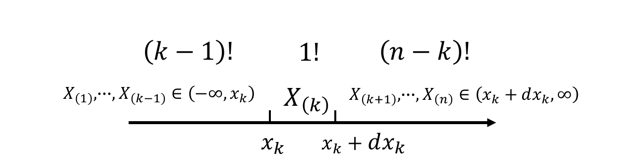
\includegraphics{2-order.png}
	\caption{次序统计量的概率微元}
	\label{Fig:order}
\end{figure}
\begin{equation}\label{Eq:ProbDiff}
	\begin{aligned}
		g({x_k}; k,n)d{x_k} = \frac{{n!}}{{(k - 1)!(n - k)!}}{[F({x_k})]^{k - 1}} f({x_k})d{x_k}{[1 - F({z_k})]^{n - k}} + o(d{x_k}) \nonumber
	\end{aligned}
\end{equation}
$g({x_k}; k,n)$即为次序统计量$X_{(k)}$的概率密度。其中,${[F({z_k})]^{k - 1}}$是前$k-1$个随机变量落入区间$(- \infty ,{x_k})$的概率;${[1 - F({x_k})]^{n - k}}$是后面$n-k$个变量落入区间$({x_k},\infty )$的概率,因为$1 - F({x_k}) = P(X > {x_k})$。 $o(d{x_k})$是$d{z_k}$的高阶无穷小量。将上式两边同时除以$d{z_k}$,则可以获得次序统计量的密度表达式
\begin{equation}
	\begin{aligned}
g({x_k};k,n) =   \frac{{n!}}{{(k - 1)!(n - k)!}} {[F({z_k})]^{k - 1}}f({x_k}){[1 - F({x_k})]^{n - k}} \nonumber
	\end{aligned}
\end{equation}
\begin{figure}[!htbp]
	\centering
	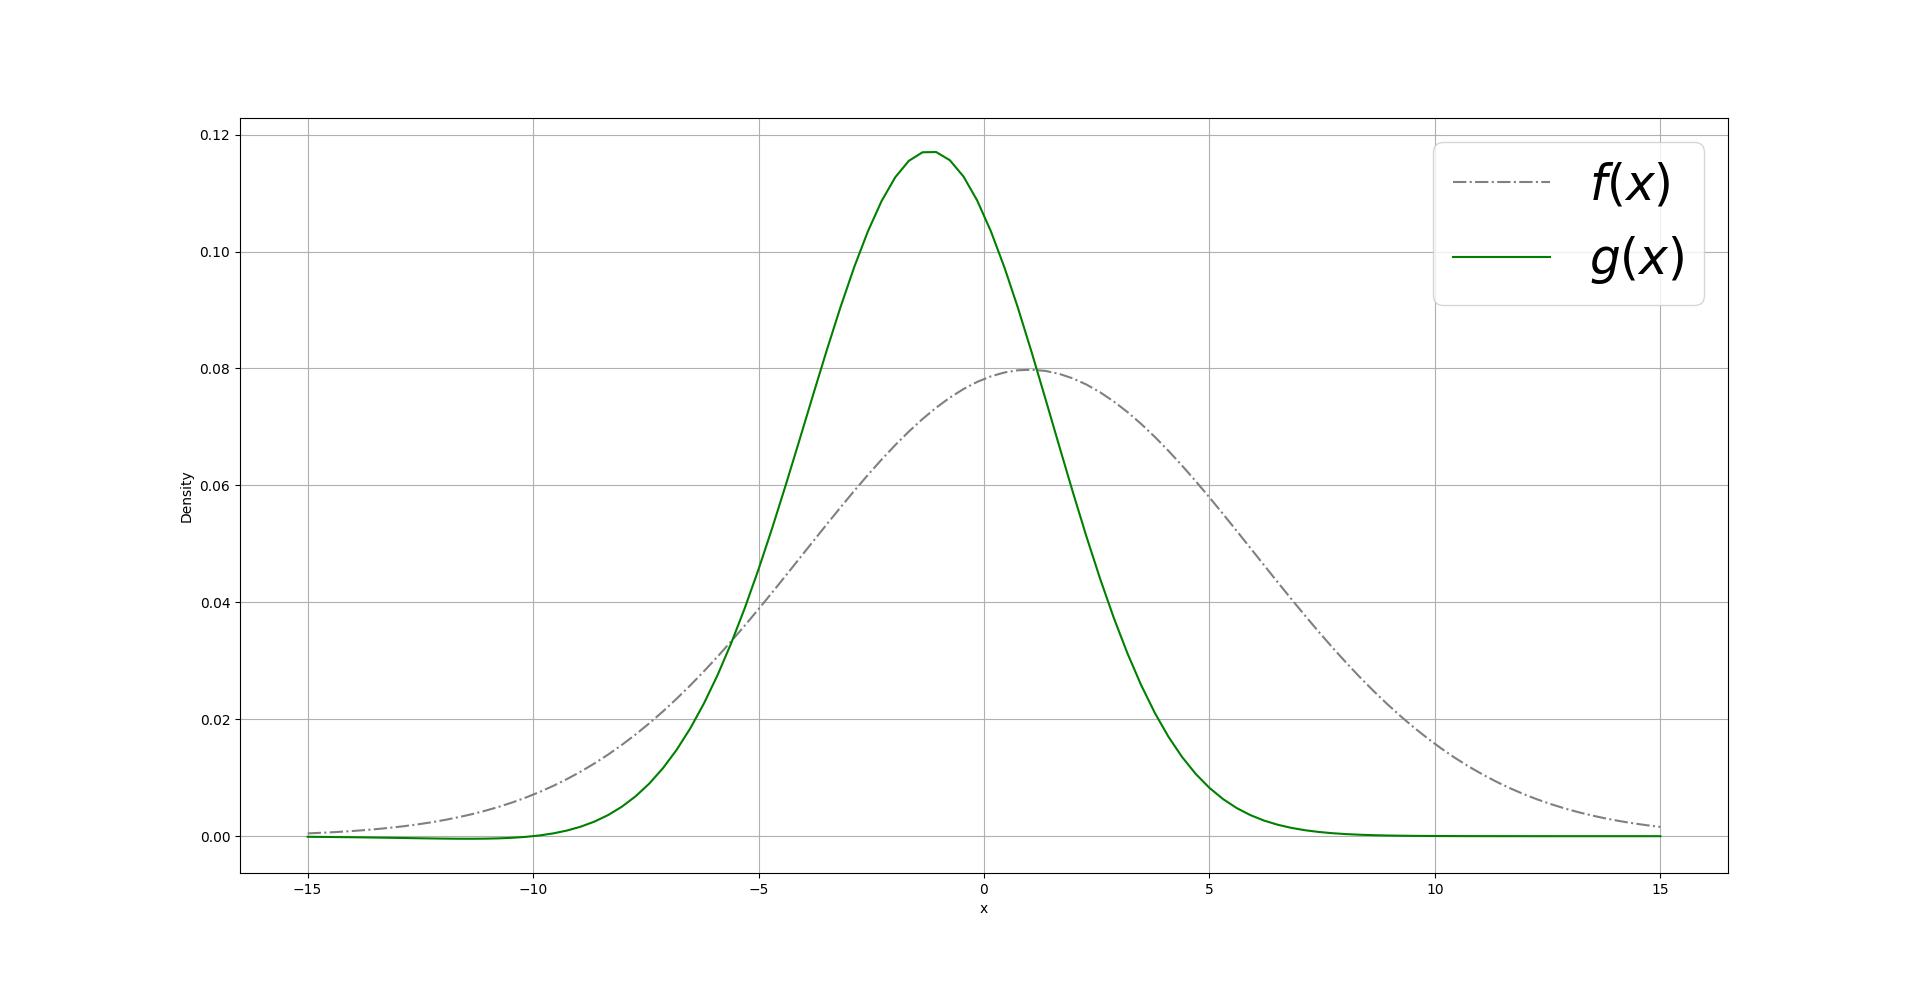
\includegraphics[width=0.6\textwidth]{order2.png}
	\caption{随机变量及其次序统计量分布示意图}
	\label{Fig:order2}
\end{figure}
上式意味着,次序统计量是随机变量分布$f(x)$的属性,只要给出随机变量的分布$f(x)$,就可以写出对应的次序统计量分布$g(x)$。图\ref{Fig:order2}给出了正态分布$\mathcal{N}(1,5)$的随机变量对应的次序统计量分布$g({x};k=2,n=5)$的示意图。可以看到,次序统计量的分布$g(x)$比$f(x)$更窄。可以使用一个例子理解这一现象:假设学生考试成绩$X$独立同分布于$f(x)$。那么在一个班级中排名最后的学生的成绩的分布可以推导为$g(x)$,其可能的成绩分数比分布$f(x)$更窄。这是因为“排名最后的学生”这个信息减少了随机变量$X$的不确定性。

如果随机变量$X$中,只包含两个总体,例如正例总体和负例总体,那么可以取$n=2$,得到次序统计量$X_{(1)}$和次序统计量$X_{(2)}$的密度为:
\begin{align}
g(x_1) &= 2 f(x) [1-F(x)] \\
g(x_2)&= 2 f(x)F(x)
\end{align}

次序统计量是非参数统计推断的最基本工具,广泛应用于诸多统计理论与实践,如分位数估计、极值分析等、排序分析等。由于个性化推荐是一个排序任务,因此次序统计量也为推荐算法提供了重要的工具。上式的两个结论,会在后面的章节多次应用。

\subsection{极大似然估计}
极大似然估计(MLE)是一种估计参数化的概率分布的方法。其基本思想是,在参数空间内,求解一个模型参数$\Theta$,使得在一次实验中观测到观测值(也称为证据)$X$的概率最大。这通过最大化似然函数来实现:
\[\arg \max p(X|\Theta)\]
其中,$p(X|\Theta)$称为似然,反映了模型参数$\Theta$对观测证据$X$的解释程度\cite{mou:2006}。以BPR为例,简单介绍极大似然估计的运作原理。给定观测到的正负样本对$X$,用户“偏好正例$i$强于负例$j$”的似然被建模为
\[p(X|\Theta) = -\log \sigma (\hat{x}_{ui} - \hat{x}_{uj})\]
其中$\hat{x}_{ui},\hat{x}_{uj}$是由用户物品特征表示$\Theta$参数化的偏好预测值。那么$p(X|\Theta)$描述了当前模型参数下,观测到用户偏好物品$i$强于$j$的概率。引入样本的独立性假设后,多个样本的似然函数是多个成对比较似然的乘积。通过对数运算将乘积运算转化为求和运算,原始的极大似然估计问题往往转化为最大化对数似然问题。

在实践中,由于要引入正则化项避免过拟合,而正则化项又等价于高斯分布先验密度的对数,因此正则化项为BPR的估计量提供了后验概率解释。
将BPR解释为极大似然估计,还是最大后验估计,主要是对正则化项的语义理解不同:若狭义地理解正则化项,那么BPR的估计量即为极大似然估计量;若把正则化项理解为高斯先验密度的对数,那么BPR为最大后验估计量。在本文成对学习的具体环境中,不区分由正则化项的语义造成的极大似然或者最大后验估计的概念差异。从贝叶斯推断的角度来看,极大似然估计通常等同于具有均匀先验分布(或标准差为无穷大的正态先验分布)的最大后验(MAP)估计\cite{beye:book}。

%极大似然通过求解参数,使得一次观测发生的概率最大化,体现的是频率学派的观点。极大似然思想也广泛体现在日常生活中,例如“要下雨(参数)了,不然不会这么闷热(观测证据)”,根据当前闷热的观测证据推断为要下雨,体现的正是极大似然原理。





